% Created by tikzDevice version 0.12.3 on 2020-12-17 10:48:51
% !TEX encoding = UTF-8 Unicode
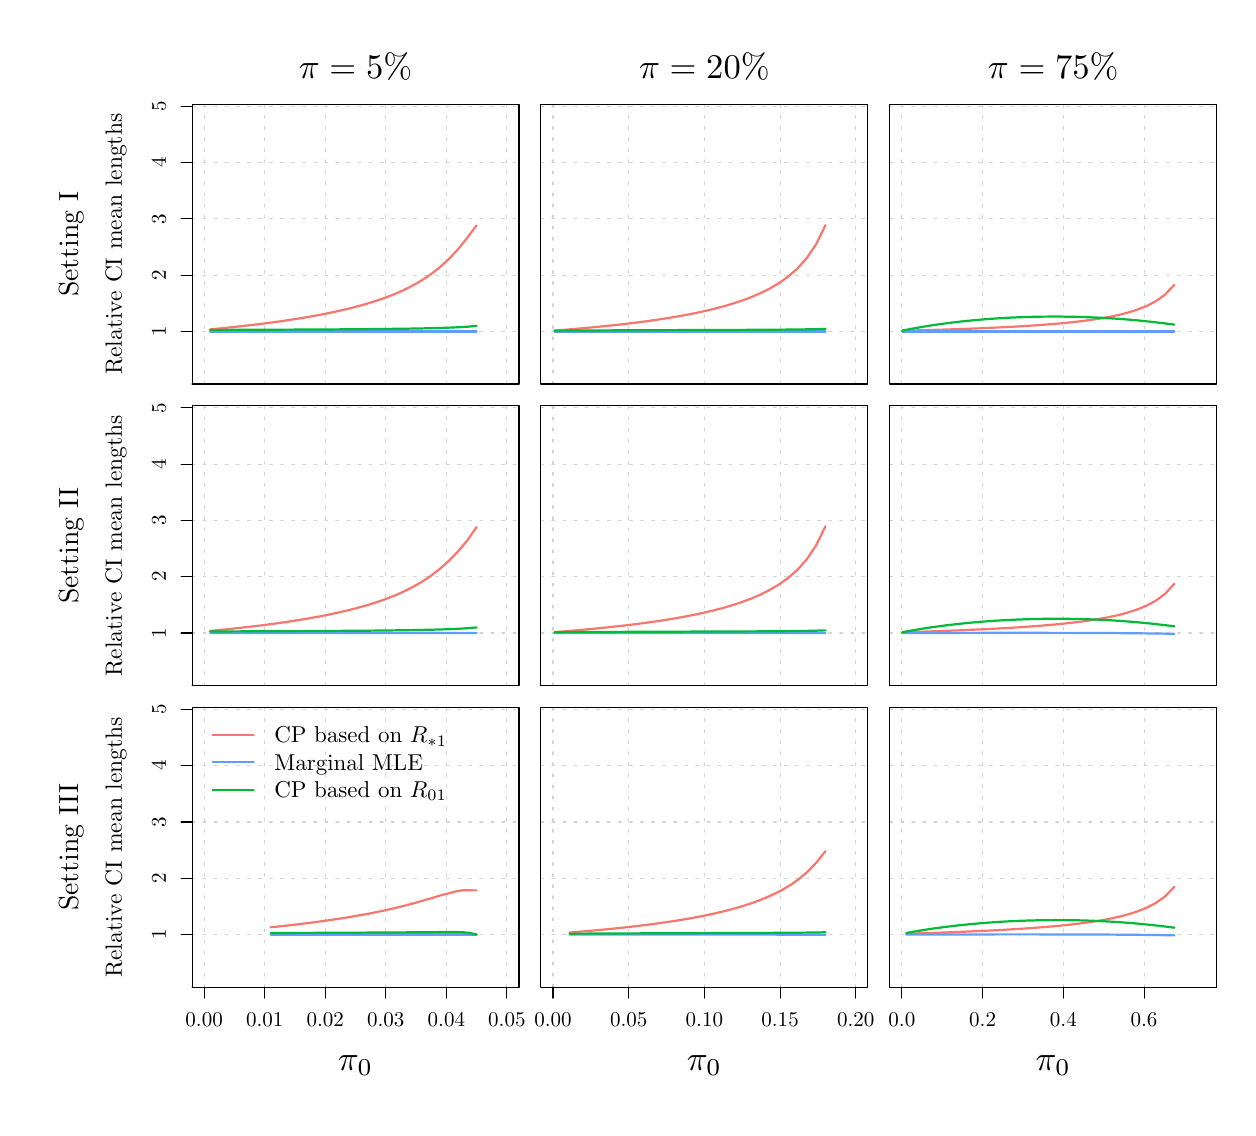
\begin{tikzpicture}[x=1pt,y=1pt]
\definecolor{fillColor}{RGB}{255,255,255}
\path[use as bounding box,fill=fillColor,fill opacity=0.00] (0,0) rectangle (433.62,390.26);
\begin{scope}
\path[clip] ( 55.44,257.53) rectangle (181.50,366.50);
\definecolor{drawColor}{RGB}{0,0,0}

\node[text=drawColor,anchor=base,inner sep=0pt, outer sep=0pt, scale=  0.66] at (118.47,231.40) {Simulation ID};

\node[text=drawColor,rotate= 90.00,anchor=base,inner sep=0pt, outer sep=0pt, scale=  0.66] at ( 34.06,312.01) {Ratio of RMSE};
\end{scope}
\begin{scope}
\path[clip] (  0.00,  0.00) rectangle (433.62,390.26);
\definecolor{drawColor}{RGB}{0,0,0}

\path[draw=drawColor,line width= 0.4pt,line join=round,line cap=round] ( 59.40,280.49) -- ( 59.40,361.85);

\path[draw=drawColor,line width= 0.4pt,line join=round,line cap=round] ( 59.40,280.49) -- ( 55.44,280.49);

\path[draw=drawColor,line width= 0.4pt,line join=round,line cap=round] ( 59.40,300.83) -- ( 55.44,300.83);

\path[draw=drawColor,line width= 0.4pt,line join=round,line cap=round] ( 59.40,321.17) -- ( 55.44,321.17);

\path[draw=drawColor,line width= 0.4pt,line join=round,line cap=round] ( 59.40,341.51) -- ( 55.44,341.51);

\path[draw=drawColor,line width= 0.4pt,line join=round,line cap=round] ( 59.40,361.85) -- ( 55.44,361.85);

\node[text=drawColor,rotate= 90.00,anchor=base,inner sep=0pt, outer sep=0pt, scale=  0.76] at ( 49.90,280.49) {1};

\node[text=drawColor,rotate= 90.00,anchor=base,inner sep=0pt, outer sep=0pt, scale=  0.76] at ( 49.90,300.83) {2};

\node[text=drawColor,rotate= 90.00,anchor=base,inner sep=0pt, outer sep=0pt, scale=  0.76] at ( 49.90,321.17) {3};

\node[text=drawColor,rotate= 90.00,anchor=base,inner sep=0pt, outer sep=0pt, scale=  0.76] at ( 49.90,341.51) {4};

\node[text=drawColor,rotate= 90.00,anchor=base,inner sep=0pt, outer sep=0pt, scale=  0.76] at ( 49.90,361.85) {5};
\end{scope}
\begin{scope}
\path[clip] ( 59.40,261.49) rectangle (177.54,362.54);
\definecolor{drawColor}{RGB}{211,211,211}

\path[draw=drawColor,line width= 0.4pt,dash pattern=on 1pt off 3pt ,line join=round,line cap=round] ( 63.78,261.49) -- ( 63.78,362.54);

\path[draw=drawColor,line width= 0.4pt,dash pattern=on 1pt off 3pt ,line join=round,line cap=round] ( 85.65,261.49) -- ( 85.65,362.54);

\path[draw=drawColor,line width= 0.4pt,dash pattern=on 1pt off 3pt ,line join=round,line cap=round] (107.53,261.49) -- (107.53,362.54);

\path[draw=drawColor,line width= 0.4pt,dash pattern=on 1pt off 3pt ,line join=round,line cap=round] (129.41,261.49) -- (129.41,362.54);

\path[draw=drawColor,line width= 0.4pt,dash pattern=on 1pt off 3pt ,line join=round,line cap=round] (151.29,261.49) -- (151.29,362.54);

\path[draw=drawColor,line width= 0.4pt,dash pattern=on 1pt off 3pt ,line join=round,line cap=round] (173.16,261.49) -- (173.16,362.54);

\path[draw=drawColor,line width= 0.4pt,dash pattern=on 1pt off 3pt ,line join=round,line cap=round] ( 59.40,280.49) -- (177.54,280.49);

\path[draw=drawColor,line width= 0.4pt,dash pattern=on 1pt off 3pt ,line join=round,line cap=round] ( 59.40,300.83) -- (177.54,300.83);

\path[draw=drawColor,line width= 0.4pt,dash pattern=on 1pt off 3pt ,line join=round,line cap=round] ( 59.40,321.17) -- (177.54,321.17);

\path[draw=drawColor,line width= 0.4pt,dash pattern=on 1pt off 3pt ,line join=round,line cap=round] ( 59.40,341.51) -- (177.54,341.51);

\path[draw=drawColor,line width= 0.4pt,dash pattern=on 1pt off 3pt ,line join=round,line cap=round] ( 59.40,361.85) -- (177.54,361.85);
\end{scope}
\begin{scope}
\path[clip] (  0.00,  0.00) rectangle (433.62,390.26);
\definecolor{drawColor}{RGB}{0,0,0}

\path[draw=drawColor,line width= 0.4pt,line join=round,line cap=round] ( 59.40,261.49) --
	(177.54,261.49) --
	(177.54,362.54) --
	( 59.40,362.54) --
	( 59.40,261.49);
\end{scope}
\begin{scope}
\path[clip] ( 59.40,261.49) rectangle (177.54,362.54);
\definecolor{drawColor}{RGB}{248,118,109}

\path[draw=drawColor,line width= 0.8pt,line join=round,line cap=round] ( 65.96,281.24) --
	( 69.28,281.56) --
	( 72.60,281.89) --
	( 75.92,282.25) --
	( 79.24,282.62) --
	( 82.56,283.01) --
	( 85.88,283.42) --
	( 89.20,283.86) --
	( 92.52,284.33) --
	( 95.84,284.82) --
	( 99.16,285.35) --
	(102.48,285.92) --
	(105.80,286.53) --
	(109.12,287.19) --
	(112.43,287.90) --
	(115.75,288.67) --
	(119.07,289.52) --
	(122.39,290.45) --
	(125.71,291.47) --
	(129.03,292.61) --
	(132.35,293.88) --
	(135.67,295.33) --
	(138.99,296.99) --
	(142.31,298.89) --
	(145.63,301.10) --
	(148.95,303.68) --
	(152.27,306.73) --
	(155.59,310.26) --
	(158.91,314.40) --
	(162.23,318.81);
\definecolor{drawColor}{RGB}{97,156,255}

\path[draw=drawColor,line width= 0.8pt,line join=round,line cap=round] ( 65.96,280.49) --
	( 69.28,280.49) --
	( 72.60,280.49) --
	( 75.92,280.49) --
	( 79.24,280.49) --
	( 82.56,280.49) --
	( 85.88,280.49) --
	( 89.20,280.49) --
	( 92.52,280.49) --
	( 95.84,280.49) --
	( 99.16,280.49) --
	(102.48,280.49) --
	(105.80,280.49) --
	(109.12,280.49) --
	(112.43,280.49) --
	(115.75,280.49) --
	(119.07,280.49) --
	(122.39,280.49) --
	(125.71,280.49) --
	(129.03,280.49) --
	(132.35,280.49) --
	(135.67,280.49) --
	(138.99,280.49) --
	(142.31,280.49) --
	(145.63,280.49) --
	(148.95,280.49) --
	(152.27,280.49) --
	(155.59,280.49) --
	(158.91,280.49) --
	(162.23,280.49);
\definecolor{drawColor}{RGB}{0,186,56}

\path[draw=drawColor,line width= 0.8pt,line join=round,line cap=round] ( 65.96,281.04) --
	( 69.28,281.05) --
	( 72.60,281.06) --
	( 75.92,281.07) --
	( 79.24,281.09) --
	( 82.56,281.10) --
	( 85.88,281.11) --
	( 89.20,281.12) --
	( 92.52,281.14) --
	( 95.84,281.15) --
	( 99.16,281.17) --
	(102.48,281.19) --
	(105.80,281.20) --
	(109.12,281.22) --
	(112.43,281.24) --
	(115.75,281.27) --
	(119.07,281.29) --
	(122.39,281.32) --
	(125.71,281.35) --
	(129.03,281.39) --
	(132.35,281.43) --
	(135.67,281.47) --
	(138.99,281.52) --
	(142.31,281.58) --
	(145.63,281.66) --
	(148.95,281.75) --
	(152.27,281.86) --
	(155.59,282.00) --
	(158.91,282.20) --
	(162.23,282.49);
\end{scope}
\begin{scope}
\path[clip] (  0.00,  0.00) rectangle (433.62,390.26);
\definecolor{drawColor}{RGB}{0,0,0}

\node[text=drawColor,rotate= 90.00,anchor=base,inner sep=0pt, outer sep=0pt, scale=  1.00] at ( 18.22,312.01) {Setting I};

\node[text=drawColor,rotate= 90.00,anchor=base,inner sep=0pt, outer sep=0pt, scale=  0.85] at ( 34.06,312.01) {Relative CI mean lengths};

\node[text=drawColor,anchor=base,inner sep=0pt, outer sep=0pt, scale=  1.25] at (118.47,372.04) {$\pi = 5\%$};
\end{scope}
\begin{scope}
\path[clip] (181.50,257.53) rectangle (307.56,366.50);
\definecolor{drawColor}{RGB}{0,0,0}

\node[text=drawColor,anchor=base,inner sep=0pt, outer sep=0pt, scale=  0.66] at (244.53,231.40) {Simulation ID};

\node[text=drawColor,rotate= 90.00,anchor=base,inner sep=0pt, outer sep=0pt, scale=  0.66] at (160.12,312.01) {Ratio of RMSE};
\end{scope}
\begin{scope}
\path[clip] (185.46,261.49) rectangle (303.60,362.54);
\definecolor{drawColor}{RGB}{211,211,211}

\path[draw=drawColor,line width= 0.4pt,dash pattern=on 1pt off 3pt ,line join=round,line cap=round] (189.84,261.49) -- (189.84,362.54);

\path[draw=drawColor,line width= 0.4pt,dash pattern=on 1pt off 3pt ,line join=round,line cap=round] (217.18,261.49) -- (217.18,362.54);

\path[draw=drawColor,line width= 0.4pt,dash pattern=on 1pt off 3pt ,line join=round,line cap=round] (244.53,261.49) -- (244.53,362.54);

\path[draw=drawColor,line width= 0.4pt,dash pattern=on 1pt off 3pt ,line join=round,line cap=round] (271.88,261.49) -- (271.88,362.54);

\path[draw=drawColor,line width= 0.4pt,dash pattern=on 1pt off 3pt ,line join=round,line cap=round] (299.22,261.49) -- (299.22,362.54);

\path[draw=drawColor,line width= 0.4pt,dash pattern=on 1pt off 3pt ,line join=round,line cap=round] (185.46,280.49) -- (303.60,280.49);

\path[draw=drawColor,line width= 0.4pt,dash pattern=on 1pt off 3pt ,line join=round,line cap=round] (185.46,300.83) -- (303.60,300.83);

\path[draw=drawColor,line width= 0.4pt,dash pattern=on 1pt off 3pt ,line join=round,line cap=round] (185.46,321.17) -- (303.60,321.17);

\path[draw=drawColor,line width= 0.4pt,dash pattern=on 1pt off 3pt ,line join=round,line cap=round] (185.46,341.51) -- (303.60,341.51);

\path[draw=drawColor,line width= 0.4pt,dash pattern=on 1pt off 3pt ,line join=round,line cap=round] (185.46,361.85) -- (303.60,361.85);
\end{scope}
\begin{scope}
\path[clip] (  0.00,  0.00) rectangle (433.62,390.26);
\definecolor{drawColor}{RGB}{0,0,0}

\path[draw=drawColor,line width= 0.4pt,line join=round,line cap=round] (185.46,261.49) --
	(303.60,261.49) --
	(303.60,362.54) --
	(185.46,362.54) --
	(185.46,261.49);
\end{scope}
\begin{scope}
\path[clip] (185.46,261.49) rectangle (303.60,362.54);
\definecolor{drawColor}{RGB}{248,118,109}

\path[draw=drawColor,line width= 0.8pt,line join=round,line cap=round] (190.38,280.81) --
	(193.76,281.07) --
	(197.13,281.35) --
	(200.51,281.64) --
	(203.89,281.95) --
	(207.26,282.28) --
	(210.64,282.62) --
	(214.01,282.99) --
	(217.39,283.39) --
	(220.77,283.80) --
	(224.14,284.25) --
	(227.52,284.73) --
	(230.89,285.25) --
	(234.27,285.81) --
	(237.65,286.41) --
	(241.02,287.07) --
	(244.40,287.79) --
	(247.77,288.59) --
	(251.15,289.47) --
	(254.53,290.46) --
	(257.90,291.56) --
	(261.28,292.81) --
	(264.65,294.25) --
	(268.03,295.92) --
	(271.41,297.90) --
	(274.78,300.28) --
	(278.16,303.23) --
	(281.53,307.00) --
	(284.91,312.00) --
	(288.29,318.89);
\definecolor{drawColor}{RGB}{97,156,255}

\path[draw=drawColor,line width= 0.8pt,line join=round,line cap=round] (190.38,280.49) --
	(193.76,280.49) --
	(197.13,280.49) --
	(200.51,280.49) --
	(203.89,280.49) --
	(207.26,280.49) --
	(210.64,280.49) --
	(214.01,280.49) --
	(217.39,280.49) --
	(220.77,280.49) --
	(224.14,280.49) --
	(227.52,280.49) --
	(230.89,280.49) --
	(234.27,280.49) --
	(237.65,280.49) --
	(241.02,280.49) --
	(244.40,280.49) --
	(247.77,280.49) --
	(251.15,280.49) --
	(254.53,280.49) --
	(257.90,280.49) --
	(261.28,280.49) --
	(264.65,280.49) --
	(268.03,280.49) --
	(271.41,280.49) --
	(274.78,280.49) --
	(278.16,280.49) --
	(281.53,280.49) --
	(284.91,280.49) --
	(288.29,280.49);
\definecolor{drawColor}{RGB}{0,186,56}

\path[draw=drawColor,line width= 0.8pt,line join=round,line cap=round] (190.38,280.77) --
	(193.76,280.79) --
	(197.13,280.81) --
	(200.51,280.83) --
	(203.89,280.84) --
	(207.26,280.86) --
	(210.64,280.88) --
	(214.01,280.89) --
	(217.39,280.90) --
	(220.77,280.92) --
	(224.14,280.93) --
	(227.52,280.94) --
	(230.89,280.96) --
	(234.27,280.97) --
	(237.65,280.98) --
	(241.02,280.99) --
	(244.40,281.00) --
	(247.77,281.02) --
	(251.15,281.03) --
	(254.53,281.04) --
	(257.90,281.05) --
	(261.28,281.07) --
	(264.65,281.09) --
	(268.03,281.11) --
	(271.41,281.13) --
	(274.78,281.16) --
	(278.16,281.20) --
	(281.53,281.25) --
	(284.91,281.32) --
	(288.29,281.43);
\end{scope}
\begin{scope}
\path[clip] (  0.00,  0.00) rectangle (433.62,390.26);
\definecolor{drawColor}{RGB}{0,0,0}

\node[text=drawColor,anchor=base,inner sep=0pt, outer sep=0pt, scale=  1.25] at (244.53,372.04) {$\pi = 20\%$};
\end{scope}
\begin{scope}
\path[clip] (307.56,257.53) rectangle (433.62,366.50);
\definecolor{drawColor}{RGB}{0,0,0}

\node[text=drawColor,anchor=base,inner sep=0pt, outer sep=0pt, scale=  0.66] at (370.59,231.40) {Simulation ID};

\node[text=drawColor,rotate= 90.00,anchor=base,inner sep=0pt, outer sep=0pt, scale=  0.66] at (286.18,312.01) {Ratio of RMSE};
\end{scope}
\begin{scope}
\path[clip] (311.52,261.49) rectangle (429.66,362.54);
\definecolor{drawColor}{RGB}{211,211,211}

\path[draw=drawColor,line width= 0.4pt,dash pattern=on 1pt off 3pt ,line join=round,line cap=round] (315.90,261.49) -- (315.90,362.54);

\path[draw=drawColor,line width= 0.4pt,dash pattern=on 1pt off 3pt ,line join=round,line cap=round] (345.07,261.49) -- (345.07,362.54);

\path[draw=drawColor,line width= 0.4pt,dash pattern=on 1pt off 3pt ,line join=round,line cap=round] (374.24,261.49) -- (374.24,362.54);

\path[draw=drawColor,line width= 0.4pt,dash pattern=on 1pt off 3pt ,line join=round,line cap=round] (403.41,261.49) -- (403.41,362.54);

\path[draw=drawColor,line width= 0.4pt,dash pattern=on 1pt off 3pt ,line join=round,line cap=round] (311.52,280.49) -- (429.66,280.49);

\path[draw=drawColor,line width= 0.4pt,dash pattern=on 1pt off 3pt ,line join=round,line cap=round] (311.52,300.83) -- (429.66,300.83);

\path[draw=drawColor,line width= 0.4pt,dash pattern=on 1pt off 3pt ,line join=round,line cap=round] (311.52,321.17) -- (429.66,321.17);

\path[draw=drawColor,line width= 0.4pt,dash pattern=on 1pt off 3pt ,line join=round,line cap=round] (311.52,341.51) -- (429.66,341.51);

\path[draw=drawColor,line width= 0.4pt,dash pattern=on 1pt off 3pt ,line join=round,line cap=round] (311.52,361.85) -- (429.66,361.85);
\end{scope}
\begin{scope}
\path[clip] (  0.00,  0.00) rectangle (433.62,390.26);
\definecolor{drawColor}{RGB}{0,0,0}

\path[draw=drawColor,line width= 0.4pt,line join=round,line cap=round] (311.52,261.49) --
	(429.66,261.49) --
	(429.66,362.54) --
	(311.52,362.54) --
	(311.52,261.49);
\end{scope}
\begin{scope}
\path[clip] (311.52,261.49) rectangle (429.66,362.54);
\definecolor{drawColor}{RGB}{248,118,109}

\path[draw=drawColor,line width= 0.8pt,line join=round,line cap=round] (316.04,280.75) --
	(319.43,280.83) --
	(322.82,280.92) --
	(326.21,281.01) --
	(329.60,281.11) --
	(332.99,281.22) --
	(336.38,281.33) --
	(339.77,281.45) --
	(343.16,281.59) --
	(346.55,281.73) --
	(349.94,281.88) --
	(353.33,282.05) --
	(356.72,282.23) --
	(360.11,282.43) --
	(363.50,282.65) --
	(366.89,282.89) --
	(370.28,283.15) --
	(373.67,283.45) --
	(377.06,283.79) --
	(380.45,284.17) --
	(383.84,284.61) --
	(387.23,285.12) --
	(390.62,285.70) --
	(394.01,286.40) --
	(397.40,287.25) --
	(400.79,288.29) --
	(404.18,289.62) --
	(407.57,291.35) --
	(410.96,293.75) --
	(414.35,297.31);
\definecolor{drawColor}{RGB}{97,156,255}

\path[draw=drawColor,line width= 0.8pt,line join=round,line cap=round] (316.04,280.49) --
	(319.43,280.49) --
	(322.82,280.49) --
	(326.21,280.49) --
	(329.60,280.49) --
	(332.99,280.49) --
	(336.38,280.49) --
	(339.77,280.49) --
	(343.16,280.49) --
	(346.55,280.49) --
	(349.94,280.49) --
	(353.33,280.49) --
	(356.72,280.49) --
	(360.11,280.49) --
	(363.50,280.49) --
	(366.89,280.49) --
	(370.28,280.49) --
	(373.67,280.49) --
	(377.06,280.49) --
	(380.45,280.49) --
	(383.84,280.49) --
	(387.23,280.49) --
	(390.62,280.49) --
	(394.01,280.49) --
	(397.40,280.49) --
	(400.79,280.49) --
	(404.18,280.49) --
	(407.57,280.49) --
	(410.96,280.49) --
	(414.35,280.49);
\definecolor{drawColor}{RGB}{0,186,56}

\path[draw=drawColor,line width= 0.8pt,line join=round,line cap=round] (316.04,280.78) --
	(319.43,281.45) --
	(322.82,282.06) --
	(326.21,282.62) --
	(329.60,283.12) --
	(332.99,283.57) --
	(336.38,283.98) --
	(339.77,284.34) --
	(343.16,284.66) --
	(346.55,284.94) --
	(349.94,285.18) --
	(353.33,285.39) --
	(356.72,285.55) --
	(360.11,285.68) --
	(363.50,285.78) --
	(366.89,285.84) --
	(370.28,285.86) --
	(373.67,285.85) --
	(377.06,285.80) --
	(380.45,285.73) --
	(383.84,285.61) --
	(387.23,285.46) --
	(390.62,285.28) --
	(394.01,285.06) --
	(397.40,284.80) --
	(400.79,284.50) --
	(404.18,284.17) --
	(407.57,283.79) --
	(410.96,283.39) --
	(414.35,282.95);
\end{scope}
\begin{scope}
\path[clip] (  0.00,  0.00) rectangle (433.62,390.26);
\definecolor{drawColor}{RGB}{0,0,0}

\node[text=drawColor,anchor=base,inner sep=0pt, outer sep=0pt, scale=  1.25] at (370.59,372.04) {$\pi = 75\%$};
\end{scope}
\begin{scope}
\path[clip] ( 55.44,148.57) rectangle (181.50,257.53);
\definecolor{drawColor}{RGB}{0,0,0}

\node[text=drawColor,anchor=base,inner sep=0pt, outer sep=0pt, scale=  0.66] at (118.47,122.43) {Simulation ID};

\node[text=drawColor,rotate= 90.00,anchor=base,inner sep=0pt, outer sep=0pt, scale=  0.66] at ( 34.06,203.05) {Ratio of RMSE};
\end{scope}
\begin{scope}
\path[clip] (  0.00,  0.00) rectangle (433.62,390.26);
\definecolor{drawColor}{RGB}{0,0,0}

\path[draw=drawColor,line width= 0.4pt,line join=round,line cap=round] ( 59.40,171.52) -- ( 59.40,252.88);

\path[draw=drawColor,line width= 0.4pt,line join=round,line cap=round] ( 59.40,171.52) -- ( 55.44,171.52);

\path[draw=drawColor,line width= 0.4pt,line join=round,line cap=round] ( 59.40,191.86) -- ( 55.44,191.86);

\path[draw=drawColor,line width= 0.4pt,line join=round,line cap=round] ( 59.40,212.20) -- ( 55.44,212.20);

\path[draw=drawColor,line width= 0.4pt,line join=round,line cap=round] ( 59.40,232.54) -- ( 55.44,232.54);

\path[draw=drawColor,line width= 0.4pt,line join=round,line cap=round] ( 59.40,252.88) -- ( 55.44,252.88);

\node[text=drawColor,rotate= 90.00,anchor=base,inner sep=0pt, outer sep=0pt, scale=  0.76] at ( 49.90,171.52) {1};

\node[text=drawColor,rotate= 90.00,anchor=base,inner sep=0pt, outer sep=0pt, scale=  0.76] at ( 49.90,191.86) {2};

\node[text=drawColor,rotate= 90.00,anchor=base,inner sep=0pt, outer sep=0pt, scale=  0.76] at ( 49.90,212.20) {3};

\node[text=drawColor,rotate= 90.00,anchor=base,inner sep=0pt, outer sep=0pt, scale=  0.76] at ( 49.90,232.54) {4};

\node[text=drawColor,rotate= 90.00,anchor=base,inner sep=0pt, outer sep=0pt, scale=  0.76] at ( 49.90,252.88) {5};
\end{scope}
\begin{scope}
\path[clip] ( 59.40,152.53) rectangle (177.54,253.57);
\definecolor{drawColor}{RGB}{211,211,211}

\path[draw=drawColor,line width= 0.4pt,dash pattern=on 1pt off 3pt ,line join=round,line cap=round] ( 63.78,152.53) -- ( 63.78,253.57);

\path[draw=drawColor,line width= 0.4pt,dash pattern=on 1pt off 3pt ,line join=round,line cap=round] ( 85.65,152.53) -- ( 85.65,253.57);

\path[draw=drawColor,line width= 0.4pt,dash pattern=on 1pt off 3pt ,line join=round,line cap=round] (107.53,152.53) -- (107.53,253.57);

\path[draw=drawColor,line width= 0.4pt,dash pattern=on 1pt off 3pt ,line join=round,line cap=round] (129.41,152.53) -- (129.41,253.57);

\path[draw=drawColor,line width= 0.4pt,dash pattern=on 1pt off 3pt ,line join=round,line cap=round] (151.29,152.53) -- (151.29,253.57);

\path[draw=drawColor,line width= 0.4pt,dash pattern=on 1pt off 3pt ,line join=round,line cap=round] (173.16,152.53) -- (173.16,253.57);

\path[draw=drawColor,line width= 0.4pt,dash pattern=on 1pt off 3pt ,line join=round,line cap=round] ( 59.40,171.52) -- (177.54,171.52);

\path[draw=drawColor,line width= 0.4pt,dash pattern=on 1pt off 3pt ,line join=round,line cap=round] ( 59.40,191.86) -- (177.54,191.86);

\path[draw=drawColor,line width= 0.4pt,dash pattern=on 1pt off 3pt ,line join=round,line cap=round] ( 59.40,212.20) -- (177.54,212.20);

\path[draw=drawColor,line width= 0.4pt,dash pattern=on 1pt off 3pt ,line join=round,line cap=round] ( 59.40,232.54) -- (177.54,232.54);

\path[draw=drawColor,line width= 0.4pt,dash pattern=on 1pt off 3pt ,line join=round,line cap=round] ( 59.40,252.88) -- (177.54,252.88);
\end{scope}
\begin{scope}
\path[clip] (  0.00,  0.00) rectangle (433.62,390.26);
\definecolor{drawColor}{RGB}{0,0,0}

\path[draw=drawColor,line width= 0.4pt,line join=round,line cap=round] ( 59.40,152.53) --
	(177.54,152.53) --
	(177.54,253.57) --
	( 59.40,253.57) --
	( 59.40,152.53);
\end{scope}
\begin{scope}
\path[clip] ( 59.40,152.53) rectangle (177.54,253.57);
\definecolor{drawColor}{RGB}{248,118,109}

\path[draw=drawColor,line width= 0.8pt,line join=round,line cap=round] ( 65.96,172.28) --
	( 69.28,172.60) --
	( 72.60,172.93) --
	( 75.92,173.29) --
	( 79.24,173.66) --
	( 82.56,174.05) --
	( 85.88,174.46) --
	( 89.20,174.90) --
	( 92.52,175.37) --
	( 95.84,175.87) --
	( 99.16,176.40) --
	(102.48,176.96) --
	(105.80,177.57) --
	(109.12,178.24) --
	(112.43,178.95) --
	(115.75,179.72) --
	(119.07,180.57) --
	(122.39,181.50) --
	(125.71,182.52) --
	(129.03,183.66) --
	(132.35,184.94) --
	(135.67,186.38) --
	(138.99,188.04) --
	(142.31,189.93) --
	(145.63,192.13) --
	(148.95,194.69) --
	(152.27,197.65) --
	(155.59,201.08) --
	(158.91,205.02) --
	(162.23,209.81);
\definecolor{drawColor}{RGB}{97,156,255}

\path[draw=drawColor,line width= 0.8pt,line join=round,line cap=round] ( 65.96,171.52) --
	( 69.28,171.52) --
	( 72.60,171.52) --
	( 75.92,171.52) --
	( 79.24,171.52) --
	( 82.56,171.52) --
	( 85.88,171.52) --
	( 89.20,171.52) --
	( 92.52,171.52) --
	( 95.84,171.52) --
	( 99.16,171.52) --
	(102.48,171.52) --
	(105.80,171.52) --
	(109.12,171.52) --
	(112.43,171.52) --
	(115.75,171.52) --
	(119.07,171.52) --
	(122.39,171.52) --
	(125.71,171.52) --
	(129.03,171.52) --
	(132.35,171.52) --
	(135.67,171.52) --
	(138.99,171.52) --
	(142.31,171.52) --
	(145.63,171.52) --
	(148.95,171.51) --
	(152.27,171.51) --
	(155.59,171.51) --
	(158.91,171.51) --
	(162.23,171.51);
\definecolor{drawColor}{RGB}{0,186,56}

\path[draw=drawColor,line width= 0.8pt,line join=round,line cap=round] ( 65.96,172.08) --
	( 69.28,172.09) --
	( 72.60,172.10) --
	( 75.92,172.11) --
	( 79.24,172.13) --
	( 82.56,172.14) --
	( 85.88,172.15) --
	( 89.20,172.16) --
	( 92.52,172.18) --
	( 95.84,172.19) --
	( 99.16,172.21) --
	(102.48,172.23) --
	(105.80,172.25) --
	(109.12,172.27) --
	(112.43,172.29) --
	(115.75,172.31) --
	(119.07,172.34) --
	(122.39,172.36) --
	(125.71,172.39) --
	(129.03,172.43) --
	(132.35,172.47) --
	(135.67,172.51) --
	(138.99,172.57) --
	(142.31,172.63) --
	(145.63,172.70) --
	(148.95,172.79) --
	(152.27,172.90) --
	(155.59,173.05) --
	(158.91,173.25) --
	(162.23,173.53);
\end{scope}
\begin{scope}
\path[clip] (  0.00,  0.00) rectangle (433.62,390.26);
\definecolor{drawColor}{RGB}{0,0,0}

\node[text=drawColor,rotate= 90.00,anchor=base,inner sep=0pt, outer sep=0pt, scale=  1.00] at ( 18.22,203.05) {Setting II};

\node[text=drawColor,rotate= 90.00,anchor=base,inner sep=0pt, outer sep=0pt, scale=  0.85] at ( 34.06,203.05) {Relative CI mean lengths};
\end{scope}
\begin{scope}
\path[clip] (181.50,148.57) rectangle (307.56,257.53);
\definecolor{drawColor}{RGB}{0,0,0}

\node[text=drawColor,anchor=base,inner sep=0pt, outer sep=0pt, scale=  0.66] at (244.53,122.43) {Simulation ID};

\node[text=drawColor,rotate= 90.00,anchor=base,inner sep=0pt, outer sep=0pt, scale=  0.66] at (160.12,203.05) {Ratio of RMSE};
\end{scope}
\begin{scope}
\path[clip] (185.46,152.53) rectangle (303.60,253.57);
\definecolor{drawColor}{RGB}{211,211,211}

\path[draw=drawColor,line width= 0.4pt,dash pattern=on 1pt off 3pt ,line join=round,line cap=round] (189.84,152.53) -- (189.84,253.57);

\path[draw=drawColor,line width= 0.4pt,dash pattern=on 1pt off 3pt ,line join=round,line cap=round] (217.18,152.53) -- (217.18,253.57);

\path[draw=drawColor,line width= 0.4pt,dash pattern=on 1pt off 3pt ,line join=round,line cap=round] (244.53,152.53) -- (244.53,253.57);

\path[draw=drawColor,line width= 0.4pt,dash pattern=on 1pt off 3pt ,line join=round,line cap=round] (271.88,152.53) -- (271.88,253.57);

\path[draw=drawColor,line width= 0.4pt,dash pattern=on 1pt off 3pt ,line join=round,line cap=round] (299.22,152.53) -- (299.22,253.57);

\path[draw=drawColor,line width= 0.4pt,dash pattern=on 1pt off 3pt ,line join=round,line cap=round] (185.46,171.52) -- (303.60,171.52);

\path[draw=drawColor,line width= 0.4pt,dash pattern=on 1pt off 3pt ,line join=round,line cap=round] (185.46,191.86) -- (303.60,191.86);

\path[draw=drawColor,line width= 0.4pt,dash pattern=on 1pt off 3pt ,line join=round,line cap=round] (185.46,212.20) -- (303.60,212.20);

\path[draw=drawColor,line width= 0.4pt,dash pattern=on 1pt off 3pt ,line join=round,line cap=round] (185.46,232.54) -- (303.60,232.54);

\path[draw=drawColor,line width= 0.4pt,dash pattern=on 1pt off 3pt ,line join=round,line cap=round] (185.46,252.88) -- (303.60,252.88);
\end{scope}
\begin{scope}
\path[clip] (  0.00,  0.00) rectangle (433.62,390.26);
\definecolor{drawColor}{RGB}{0,0,0}

\path[draw=drawColor,line width= 0.4pt,line join=round,line cap=round] (185.46,152.53) --
	(303.60,152.53) --
	(303.60,253.57) --
	(185.46,253.57) --
	(185.46,152.53);
\end{scope}
\begin{scope}
\path[clip] (185.46,152.53) rectangle (303.60,253.57);
\definecolor{drawColor}{RGB}{248,118,109}

\path[draw=drawColor,line width= 0.8pt,line join=round,line cap=round] (190.38,171.85) --
	(193.76,172.11) --
	(197.13,172.39) --
	(200.51,172.69) --
	(203.89,173.00) --
	(207.26,173.33) --
	(210.64,173.67) --
	(214.01,174.04) --
	(217.39,174.44) --
	(220.77,174.86) --
	(224.14,175.31) --
	(227.52,175.79) --
	(230.89,176.31) --
	(234.27,176.87) --
	(237.65,177.48) --
	(241.02,178.14) --
	(244.40,178.87) --
	(247.77,179.66) --
	(251.15,180.55) --
	(254.53,181.53) --
	(257.90,182.64) --
	(261.28,183.90) --
	(264.65,185.34) --
	(268.03,187.03) --
	(271.41,189.01) --
	(274.78,191.40) --
	(278.16,194.36) --
	(281.53,198.15) --
	(284.91,203.17) --
	(288.29,210.09);
\definecolor{drawColor}{RGB}{97,156,255}

\path[draw=drawColor,line width= 0.8pt,line join=round,line cap=round] (190.38,171.52) --
	(193.76,171.52) --
	(197.13,171.52) --
	(200.51,171.52) --
	(203.89,171.52) --
	(207.26,171.52) --
	(210.64,171.52) --
	(214.01,171.52) --
	(217.39,171.51) --
	(220.77,171.51) --
	(224.14,171.51) --
	(227.52,171.51) --
	(230.89,171.51) --
	(234.27,171.51) --
	(237.65,171.51) --
	(241.02,171.50) --
	(244.40,171.50) --
	(247.77,171.50) --
	(251.15,171.50) --
	(254.53,171.50) --
	(257.90,171.50) --
	(261.28,171.50) --
	(264.65,171.49) --
	(268.03,171.49) --
	(271.41,171.49) --
	(274.78,171.49) --
	(278.16,171.49) --
	(281.53,171.48) --
	(284.91,171.48) --
	(288.29,171.48);
\definecolor{drawColor}{RGB}{0,186,56}

\path[draw=drawColor,line width= 0.8pt,line join=round,line cap=round] (190.38,171.81) --
	(193.76,171.83) --
	(197.13,171.85) --
	(200.51,171.86) --
	(203.89,171.88) --
	(207.26,171.90) --
	(210.64,171.91) --
	(214.01,171.93) --
	(217.39,171.94) --
	(220.77,171.95) --
	(224.14,171.97) --
	(227.52,171.98) --
	(230.89,171.99) --
	(234.27,172.00) --
	(237.65,172.02) --
	(241.02,172.03) --
	(244.40,172.04) --
	(247.77,172.05) --
	(251.15,172.06) --
	(254.53,172.08) --
	(257.90,172.09) --
	(261.28,172.11) --
	(264.65,172.12) --
	(268.03,172.14) --
	(271.41,172.17) --
	(274.78,172.20) --
	(278.16,172.24) --
	(281.53,172.29) --
	(284.91,172.36) --
	(288.29,172.48);
\end{scope}
\begin{scope}
\path[clip] (307.56,148.57) rectangle (433.62,257.53);
\definecolor{drawColor}{RGB}{0,0,0}

\node[text=drawColor,anchor=base,inner sep=0pt, outer sep=0pt, scale=  0.66] at (370.59,122.43) {Simulation ID};

\node[text=drawColor,rotate= 90.00,anchor=base,inner sep=0pt, outer sep=0pt, scale=  0.66] at (286.18,203.05) {Ratio of RMSE};
\end{scope}
\begin{scope}
\path[clip] (311.52,152.53) rectangle (429.66,253.57);
\definecolor{drawColor}{RGB}{211,211,211}

\path[draw=drawColor,line width= 0.4pt,dash pattern=on 1pt off 3pt ,line join=round,line cap=round] (315.90,152.53) -- (315.90,253.57);

\path[draw=drawColor,line width= 0.4pt,dash pattern=on 1pt off 3pt ,line join=round,line cap=round] (345.07,152.53) -- (345.07,253.57);

\path[draw=drawColor,line width= 0.4pt,dash pattern=on 1pt off 3pt ,line join=round,line cap=round] (374.24,152.53) -- (374.24,253.57);

\path[draw=drawColor,line width= 0.4pt,dash pattern=on 1pt off 3pt ,line join=round,line cap=round] (403.41,152.53) -- (403.41,253.57);

\path[draw=drawColor,line width= 0.4pt,dash pattern=on 1pt off 3pt ,line join=round,line cap=round] (311.52,171.52) -- (429.66,171.52);

\path[draw=drawColor,line width= 0.4pt,dash pattern=on 1pt off 3pt ,line join=round,line cap=round] (311.52,191.86) -- (429.66,191.86);

\path[draw=drawColor,line width= 0.4pt,dash pattern=on 1pt off 3pt ,line join=round,line cap=round] (311.52,212.20) -- (429.66,212.20);

\path[draw=drawColor,line width= 0.4pt,dash pattern=on 1pt off 3pt ,line join=round,line cap=round] (311.52,232.54) -- (429.66,232.54);

\path[draw=drawColor,line width= 0.4pt,dash pattern=on 1pt off 3pt ,line join=round,line cap=round] (311.52,252.88) -- (429.66,252.88);
\end{scope}
\begin{scope}
\path[clip] (  0.00,  0.00) rectangle (433.62,390.26);
\definecolor{drawColor}{RGB}{0,0,0}

\path[draw=drawColor,line width= 0.4pt,line join=round,line cap=round] (311.52,152.53) --
	(429.66,152.53) --
	(429.66,253.57) --
	(311.52,253.57) --
	(311.52,152.53);
\end{scope}
\begin{scope}
\path[clip] (311.52,152.53) rectangle (429.66,253.57);
\definecolor{drawColor}{RGB}{248,118,109}

\path[draw=drawColor,line width= 0.8pt,line join=round,line cap=round] (316.04,171.78) --
	(319.43,171.88) --
	(322.82,171.99) --
	(326.21,172.10) --
	(329.60,172.22) --
	(332.99,172.34) --
	(336.38,172.47) --
	(339.77,172.62) --
	(343.16,172.77) --
	(346.55,172.93) --
	(349.94,173.10) --
	(353.33,173.29) --
	(356.72,173.49) --
	(360.11,173.71) --
	(363.50,173.96) --
	(366.89,174.22) --
	(370.28,174.51) --
	(373.67,174.84) --
	(377.06,175.20) --
	(380.45,175.61) --
	(383.84,176.08) --
	(387.23,176.62) --
	(390.62,177.24) --
	(394.01,177.98) --
	(397.40,178.87) --
	(400.79,179.96) --
	(404.18,181.34) --
	(407.57,183.15) --
	(410.96,185.64) --
	(414.35,189.31);
\definecolor{drawColor}{RGB}{97,156,255}

\path[draw=drawColor,line width= 0.8pt,line join=round,line cap=round] (316.04,171.52) --
	(319.43,171.53) --
	(322.82,171.54) --
	(326.21,171.55) --
	(329.60,171.55) --
	(332.99,171.56) --
	(336.38,171.56) --
	(339.77,171.57) --
	(343.16,171.57) --
	(346.55,171.58) --
	(349.94,171.58) --
	(353.33,171.58) --
	(356.72,171.58) --
	(360.11,171.58) --
	(363.50,171.58) --
	(366.89,171.58) --
	(370.28,171.57) --
	(373.67,171.57) --
	(377.06,171.56) --
	(380.45,171.55) --
	(383.84,171.54) --
	(387.23,171.52) --
	(390.62,171.50) --
	(394.01,171.48) --
	(397.40,171.45) --
	(400.79,171.42) --
	(404.18,171.38) --
	(407.57,171.34) --
	(410.96,171.29) --
	(414.35,171.23);
\definecolor{drawColor}{RGB}{0,186,56}

\path[draw=drawColor,line width= 0.8pt,line join=round,line cap=round] (316.04,171.80) --
	(319.43,172.43) --
	(322.82,173.00) --
	(326.21,173.52) --
	(329.60,173.99) --
	(332.99,174.42) --
	(336.38,174.81) --
	(339.77,175.16) --
	(343.16,175.47) --
	(346.55,175.74) --
	(349.94,175.98) --
	(353.33,176.18) --
	(356.72,176.34) --
	(360.11,176.47) --
	(363.50,176.57) --
	(366.89,176.64) --
	(370.28,176.67) --
	(373.67,176.67) --
	(377.06,176.63) --
	(380.45,176.57) --
	(383.84,176.46) --
	(387.23,176.33) --
	(390.62,176.16) --
	(394.01,175.95) --
	(397.40,175.70) --
	(400.79,175.42) --
	(404.18,175.11) --
	(407.57,174.75) --
	(410.96,174.36) --
	(414.35,173.94);
\end{scope}
\begin{scope}
\path[clip] ( 55.44, 39.60) rectangle (181.50,148.57);
\definecolor{drawColor}{RGB}{0,0,0}

\node[text=drawColor,anchor=base,inner sep=0pt, outer sep=0pt, scale=  0.66] at (118.47, 13.46) {Simulation ID};

\node[text=drawColor,rotate= 90.00,anchor=base,inner sep=0pt, outer sep=0pt, scale=  0.66] at ( 34.06, 94.08) {Ratio of RMSE};
\end{scope}
\begin{scope}
\path[clip] (  0.00,  0.00) rectangle (433.62,390.26);
\definecolor{drawColor}{RGB}{0,0,0}

\path[draw=drawColor,line width= 0.4pt,line join=round,line cap=round] ( 59.40, 62.56) -- ( 59.40,143.91);

\path[draw=drawColor,line width= 0.4pt,line join=round,line cap=round] ( 59.40, 62.56) -- ( 55.44, 62.56);

\path[draw=drawColor,line width= 0.4pt,line join=round,line cap=round] ( 59.40, 82.90) -- ( 55.44, 82.90);

\path[draw=drawColor,line width= 0.4pt,line join=round,line cap=round] ( 59.40,103.24) -- ( 55.44,103.24);

\path[draw=drawColor,line width= 0.4pt,line join=round,line cap=round] ( 59.40,123.58) -- ( 55.44,123.58);

\path[draw=drawColor,line width= 0.4pt,line join=round,line cap=round] ( 59.40,143.91) -- ( 55.44,143.91);

\node[text=drawColor,rotate= 90.00,anchor=base,inner sep=0pt, outer sep=0pt, scale=  0.76] at ( 49.90, 62.56) {1};

\node[text=drawColor,rotate= 90.00,anchor=base,inner sep=0pt, outer sep=0pt, scale=  0.76] at ( 49.90, 82.90) {2};

\node[text=drawColor,rotate= 90.00,anchor=base,inner sep=0pt, outer sep=0pt, scale=  0.76] at ( 49.90,103.24) {3};

\node[text=drawColor,rotate= 90.00,anchor=base,inner sep=0pt, outer sep=0pt, scale=  0.76] at ( 49.90,123.58) {4};

\node[text=drawColor,rotate= 90.00,anchor=base,inner sep=0pt, outer sep=0pt, scale=  0.76] at ( 49.90,143.91) {5};
\end{scope}
\begin{scope}
\path[clip] ( 59.40, 43.56) rectangle (177.54,144.61);
\definecolor{drawColor}{RGB}{211,211,211}

\path[draw=drawColor,line width= 0.4pt,dash pattern=on 1pt off 3pt ,line join=round,line cap=round] ( 63.78, 43.56) -- ( 63.78,144.61);

\path[draw=drawColor,line width= 0.4pt,dash pattern=on 1pt off 3pt ,line join=round,line cap=round] ( 85.65, 43.56) -- ( 85.65,144.61);

\path[draw=drawColor,line width= 0.4pt,dash pattern=on 1pt off 3pt ,line join=round,line cap=round] (107.53, 43.56) -- (107.53,144.61);

\path[draw=drawColor,line width= 0.4pt,dash pattern=on 1pt off 3pt ,line join=round,line cap=round] (129.41, 43.56) -- (129.41,144.61);

\path[draw=drawColor,line width= 0.4pt,dash pattern=on 1pt off 3pt ,line join=round,line cap=round] (151.29, 43.56) -- (151.29,144.61);

\path[draw=drawColor,line width= 0.4pt,dash pattern=on 1pt off 3pt ,line join=round,line cap=round] (173.16, 43.56) -- (173.16,144.61);

\path[draw=drawColor,line width= 0.4pt,dash pattern=on 1pt off 3pt ,line join=round,line cap=round] ( 59.40, 62.56) -- (177.54, 62.56);

\path[draw=drawColor,line width= 0.4pt,dash pattern=on 1pt off 3pt ,line join=round,line cap=round] ( 59.40, 82.90) -- (177.54, 82.90);

\path[draw=drawColor,line width= 0.4pt,dash pattern=on 1pt off 3pt ,line join=round,line cap=round] ( 59.40,103.24) -- (177.54,103.24);

\path[draw=drawColor,line width= 0.4pt,dash pattern=on 1pt off 3pt ,line join=round,line cap=round] ( 59.40,123.58) -- (177.54,123.58);

\path[draw=drawColor,line width= 0.4pt,dash pattern=on 1pt off 3pt ,line join=round,line cap=round] ( 59.40,143.91) -- (177.54,143.91);
\end{scope}
\begin{scope}
\path[clip] (  0.00,  0.00) rectangle (433.62,390.26);
\definecolor{drawColor}{RGB}{0,0,0}

\path[draw=drawColor,line width= 0.4pt,line join=round,line cap=round] ( 63.78, 43.56) -- (173.16, 43.56);

\path[draw=drawColor,line width= 0.4pt,line join=round,line cap=round] ( 63.78, 43.56) -- ( 63.78, 39.60);

\path[draw=drawColor,line width= 0.4pt,line join=round,line cap=round] ( 85.65, 43.56) -- ( 85.65, 39.60);

\path[draw=drawColor,line width= 0.4pt,line join=round,line cap=round] (107.53, 43.56) -- (107.53, 39.60);

\path[draw=drawColor,line width= 0.4pt,line join=round,line cap=round] (129.41, 43.56) -- (129.41, 39.60);

\path[draw=drawColor,line width= 0.4pt,line join=round,line cap=round] (151.29, 43.56) -- (151.29, 39.60);

\path[draw=drawColor,line width= 0.4pt,line join=round,line cap=round] (173.16, 43.56) -- (173.16, 39.60);

\node[text=drawColor,anchor=base,inner sep=0pt, outer sep=0pt, scale=  0.76] at ( 63.78, 29.30) {0.00};

\node[text=drawColor,anchor=base,inner sep=0pt, outer sep=0pt, scale=  0.76] at ( 85.65, 29.30) {0.01};

\node[text=drawColor,anchor=base,inner sep=0pt, outer sep=0pt, scale=  0.76] at (107.53, 29.30) {0.02};

\node[text=drawColor,anchor=base,inner sep=0pt, outer sep=0pt, scale=  0.76] at (129.41, 29.30) {0.03};

\node[text=drawColor,anchor=base,inner sep=0pt, outer sep=0pt, scale=  0.76] at (151.29, 29.30) {0.04};

\node[text=drawColor,anchor=base,inner sep=0pt, outer sep=0pt, scale=  0.76] at (173.16, 29.30) {0.05};

\path[draw=drawColor,line width= 0.4pt,line join=round,line cap=round] ( 59.40, 43.56) --
	(177.54, 43.56) --
	(177.54,144.61) --
	( 59.40,144.61) --
	( 59.40, 43.56);
\end{scope}
\begin{scope}
\path[clip] ( 59.40, 43.56) rectangle (177.54,144.61);
\definecolor{drawColor}{RGB}{248,118,109}

\path[draw=drawColor,line width= 0.8pt,line join=round,line cap=round] ( 87.84, 65.18) --
	( 90.41, 65.45) --
	( 92.97, 65.73) --
	( 95.54, 66.01) --
	( 98.10, 66.31) --
	(100.67, 66.63) --
	(103.23, 66.96) --
	(105.80, 67.30) --
	(108.36, 67.66) --
	(110.93, 68.04) --
	(113.49, 68.43) --
	(116.06, 68.84) --
	(118.62, 69.28) --
	(121.19, 69.73) --
	(123.75, 70.21) --
	(126.32, 70.72) --
	(128.88, 71.26) --
	(131.45, 71.83) --
	(134.01, 72.44) --
	(136.58, 73.08) --
	(139.14, 73.76) --
	(141.71, 74.48) --
	(144.27, 75.23) --
	(146.84, 75.98) --
	(149.40, 76.77) --
	(151.97, 77.39) --
	(154.53, 78.09) --
	(157.10, 78.57) --
	(159.66, 78.53) --
	(162.23, 78.52);
\definecolor{drawColor}{RGB}{97,156,255}

\path[draw=drawColor,line width= 0.8pt,line join=round,line cap=round] ( 87.84, 62.55) --
	( 90.41, 62.55) --
	( 92.97, 62.55) --
	( 95.54, 62.55) --
	( 98.10, 62.55) --
	(100.67, 62.55) --
	(103.23, 62.55) --
	(105.80, 62.55) --
	(108.36, 62.55) --
	(110.93, 62.55) --
	(113.49, 62.55) --
	(116.06, 62.55) --
	(118.62, 62.55) --
	(121.19, 62.55) --
	(123.75, 62.55) --
	(126.32, 62.55) --
	(128.88, 62.55) --
	(131.45, 62.55) --
	(134.01, 62.55) --
	(136.58, 62.55) --
	(139.14, 62.55) --
	(141.71, 62.55) --
	(144.27, 62.55) --
	(146.84, 62.55) --
	(149.40, 62.55) --
	(151.97, 62.55) --
	(154.53, 62.55) --
	(157.10, 62.55) --
	(159.66, 62.55) --
	(162.23, 62.55);
\definecolor{drawColor}{RGB}{0,186,56}

\path[draw=drawColor,line width= 0.8pt,line join=round,line cap=round] ( 87.84, 63.12) --
	( 90.41, 63.13) --
	( 92.97, 63.14) --
	( 95.54, 63.15) --
	( 98.10, 63.16) --
	(100.67, 63.17) --
	(103.23, 63.17) --
	(105.80, 63.18) --
	(108.36, 63.19) --
	(110.93, 63.21) --
	(113.49, 63.22) --
	(116.06, 63.23) --
	(118.62, 63.24) --
	(121.19, 63.25) --
	(123.75, 63.27) --
	(126.32, 63.28) --
	(128.88, 63.29) --
	(131.45, 63.31) --
	(134.01, 63.33) --
	(136.58, 63.35) --
	(139.14, 63.37) --
	(141.71, 63.39) --
	(144.27, 63.41) --
	(146.84, 63.43) --
	(149.40, 63.46) --
	(151.97, 63.47) --
	(154.53, 63.47) --
	(157.10, 63.41) --
	(159.66, 63.16) --
	(162.23, 62.56);
\end{scope}
\begin{scope}
\path[clip] (  0.00,  0.00) rectangle (433.62,390.26);
\definecolor{drawColor}{RGB}{0,0,0}

\node[text=drawColor,rotate= 90.00,anchor=base,inner sep=0pt, outer sep=0pt, scale=  1.00] at ( 18.22, 94.08) {Setting III};

\node[text=drawColor,rotate= 90.00,anchor=base,inner sep=0pt, outer sep=0pt, scale=  0.85] at ( 34.06, 94.08) {Relative CI mean lengths};

\node[text=drawColor,anchor=base,inner sep=0pt, outer sep=0pt, scale=  1.25] at (118.47, 13.46) {$\pi_0$};
\end{scope}
\begin{scope}
\path[clip] ( 59.40, 43.56) rectangle (177.54,144.61);
\definecolor{drawColor}{RGB}{248,118,109}

\path[draw=drawColor,line width= 0.8pt,line join=round,line cap=round] ( 66.83,134.71) -- ( 81.67,134.71);
\definecolor{drawColor}{RGB}{97,156,255}

\path[draw=drawColor,line width= 0.8pt,line join=round,line cap=round] ( 66.83,124.81) -- ( 81.67,124.81);
\definecolor{drawColor}{RGB}{0,186,56}

\path[draw=drawColor,line width= 0.8pt,line join=round,line cap=round] ( 66.83,114.91) -- ( 81.67,114.91);
\definecolor{drawColor}{RGB}{0,0,0}

\node[text=drawColor,anchor=base west,inner sep=0pt, outer sep=0pt, scale=  0.83] at ( 89.10,131.87) {CP based on $R_{\ast1}$};

\node[text=drawColor,anchor=base west,inner sep=0pt, outer sep=0pt, scale=  0.83] at ( 89.10,121.97) {Marginal MLE};

\node[text=drawColor,anchor=base west,inner sep=0pt, outer sep=0pt, scale=  0.83] at ( 89.10,112.07) {CP based on $R_{01}$};
\end{scope}
\begin{scope}
\path[clip] (181.50, 39.60) rectangle (307.56,148.57);
\definecolor{drawColor}{RGB}{0,0,0}

\node[text=drawColor,anchor=base,inner sep=0pt, outer sep=0pt, scale=  0.66] at (244.53, 13.46) {Simulation ID};

\node[text=drawColor,rotate= 90.00,anchor=base,inner sep=0pt, outer sep=0pt, scale=  0.66] at (160.12, 94.08) {Ratio of RMSE};
\end{scope}
\begin{scope}
\path[clip] (185.46, 43.56) rectangle (303.60,144.61);
\definecolor{drawColor}{RGB}{211,211,211}

\path[draw=drawColor,line width= 0.4pt,dash pattern=on 1pt off 3pt ,line join=round,line cap=round] (189.84, 43.56) -- (189.84,144.61);

\path[draw=drawColor,line width= 0.4pt,dash pattern=on 1pt off 3pt ,line join=round,line cap=round] (217.18, 43.56) -- (217.18,144.61);

\path[draw=drawColor,line width= 0.4pt,dash pattern=on 1pt off 3pt ,line join=round,line cap=round] (244.53, 43.56) -- (244.53,144.61);

\path[draw=drawColor,line width= 0.4pt,dash pattern=on 1pt off 3pt ,line join=round,line cap=round] (271.88, 43.56) -- (271.88,144.61);

\path[draw=drawColor,line width= 0.4pt,dash pattern=on 1pt off 3pt ,line join=round,line cap=round] (299.22, 43.56) -- (299.22,144.61);

\path[draw=drawColor,line width= 0.4pt,dash pattern=on 1pt off 3pt ,line join=round,line cap=round] (185.46, 62.56) -- (303.60, 62.56);

\path[draw=drawColor,line width= 0.4pt,dash pattern=on 1pt off 3pt ,line join=round,line cap=round] (185.46, 82.90) -- (303.60, 82.90);

\path[draw=drawColor,line width= 0.4pt,dash pattern=on 1pt off 3pt ,line join=round,line cap=round] (185.46,103.24) -- (303.60,103.24);

\path[draw=drawColor,line width= 0.4pt,dash pattern=on 1pt off 3pt ,line join=round,line cap=round] (185.46,123.58) -- (303.60,123.58);

\path[draw=drawColor,line width= 0.4pt,dash pattern=on 1pt off 3pt ,line join=round,line cap=round] (185.46,143.91) -- (303.60,143.91);
\end{scope}
\begin{scope}
\path[clip] (  0.00,  0.00) rectangle (433.62,390.26);
\definecolor{drawColor}{RGB}{0,0,0}

\path[draw=drawColor,line width= 0.4pt,line join=round,line cap=round] (185.46, 43.56) --
	(303.60, 43.56) --
	(303.60,144.61) --
	(185.46,144.61) --
	(185.46, 43.56);

\path[draw=drawColor,line width= 0.4pt,line join=round,line cap=round] (189.84, 43.56) -- (299.22, 43.56);

\path[draw=drawColor,line width= 0.4pt,line join=round,line cap=round] (189.84, 43.56) -- (189.84, 39.60);

\path[draw=drawColor,line width= 0.4pt,line join=round,line cap=round] (217.18, 43.56) -- (217.18, 39.60);

\path[draw=drawColor,line width= 0.4pt,line join=round,line cap=round] (244.53, 43.56) -- (244.53, 39.60);

\path[draw=drawColor,line width= 0.4pt,line join=round,line cap=round] (271.88, 43.56) -- (271.88, 39.60);

\path[draw=drawColor,line width= 0.4pt,line join=round,line cap=round] (299.22, 43.56) -- (299.22, 39.60);

\node[text=drawColor,anchor=base,inner sep=0pt, outer sep=0pt, scale=  0.76] at (189.84, 29.30) {0.00};

\node[text=drawColor,anchor=base,inner sep=0pt, outer sep=0pt, scale=  0.76] at (217.18, 29.30) {0.05};

\node[text=drawColor,anchor=base,inner sep=0pt, outer sep=0pt, scale=  0.76] at (244.53, 29.30) {0.10};

\node[text=drawColor,anchor=base,inner sep=0pt, outer sep=0pt, scale=  0.76] at (271.88, 29.30) {0.15};

\node[text=drawColor,anchor=base,inner sep=0pt, outer sep=0pt, scale=  0.76] at (299.22, 29.30) {0.20};
\end{scope}
\begin{scope}
\path[clip] (185.46, 43.56) rectangle (303.60,144.61);
\definecolor{drawColor}{RGB}{248,118,109}

\path[draw=drawColor,line width= 0.8pt,line join=round,line cap=round] (195.85, 63.29) --
	(199.04, 63.55) --
	(202.23, 63.82) --
	(205.41, 64.10) --
	(208.60, 64.40) --
	(211.79, 64.71) --
	(214.98, 65.05) --
	(218.16, 65.40) --
	(221.35, 65.77) --
	(224.54, 66.17) --
	(227.73, 66.59) --
	(230.91, 67.05) --
	(234.10, 67.53) --
	(237.29, 68.05) --
	(240.48, 68.61) --
	(243.66, 69.22) --
	(246.85, 69.88) --
	(250.04, 70.60) --
	(253.22, 71.39) --
	(256.41, 72.26) --
	(259.60, 73.23) --
	(262.79, 74.31) --
	(265.97, 75.53) --
	(269.16, 76.92) --
	(272.35, 78.53) --
	(275.54, 80.40) --
	(278.72, 82.63) --
	(281.91, 85.35) --
	(285.10, 88.71) --
	(288.29, 92.72);
\definecolor{drawColor}{RGB}{97,156,255}

\path[draw=drawColor,line width= 0.8pt,line join=round,line cap=round] (195.85, 62.56) --
	(199.04, 62.55) --
	(202.23, 62.55) --
	(205.41, 62.55) --
	(208.60, 62.55) --
	(211.79, 62.55) --
	(214.98, 62.55) --
	(218.16, 62.55) --
	(221.35, 62.55) --
	(224.54, 62.55) --
	(227.73, 62.54) --
	(230.91, 62.54) --
	(234.10, 62.54) --
	(237.29, 62.54) --
	(240.48, 62.54) --
	(243.66, 62.54) --
	(246.85, 62.54) --
	(250.04, 62.53) --
	(253.22, 62.53) --
	(256.41, 62.53) --
	(259.60, 62.53) --
	(262.79, 62.53) --
	(265.97, 62.53) --
	(269.16, 62.53) --
	(272.35, 62.52) --
	(275.54, 62.52) --
	(278.72, 62.52) --
	(281.91, 62.52) --
	(285.10, 62.52) --
	(288.29, 62.51);
\definecolor{drawColor}{RGB}{0,186,56}

\path[draw=drawColor,line width= 0.8pt,line join=round,line cap=round] (195.85, 62.87) --
	(199.04, 62.89) --
	(202.23, 62.90) --
	(205.41, 62.92) --
	(208.60, 62.93) --
	(211.79, 62.95) --
	(214.98, 62.96) --
	(218.16, 62.98) --
	(221.35, 62.99) --
	(224.54, 63.00) --
	(227.73, 63.01) --
	(230.91, 63.02) --
	(234.10, 63.04) --
	(237.29, 63.05) --
	(240.48, 63.06) --
	(243.66, 63.07) --
	(246.85, 63.08) --
	(250.04, 63.09) --
	(253.22, 63.10) --
	(256.41, 63.11) --
	(259.60, 63.12) --
	(262.79, 63.14) --
	(265.97, 63.15) --
	(269.16, 63.17) --
	(272.35, 63.18) --
	(275.54, 63.21) --
	(278.72, 63.23) --
	(281.91, 63.27) --
	(285.10, 63.31) --
	(288.29, 63.38);
\end{scope}
\begin{scope}
\path[clip] (  0.00,  0.00) rectangle (433.62,390.26);
\definecolor{drawColor}{RGB}{0,0,0}

\node[text=drawColor,anchor=base,inner sep=0pt, outer sep=0pt, scale=  1.25] at (244.53, 13.46) {$\pi_0$};
\end{scope}
\begin{scope}
\path[clip] (307.56, 39.60) rectangle (433.62,148.57);
\definecolor{drawColor}{RGB}{0,0,0}

\node[text=drawColor,anchor=base,inner sep=0pt, outer sep=0pt, scale=  0.66] at (370.59, 13.46) {Simulation ID};

\node[text=drawColor,rotate= 90.00,anchor=base,inner sep=0pt, outer sep=0pt, scale=  0.66] at (286.18, 94.08) {Ratio of RMSE};
\end{scope}
\begin{scope}
\path[clip] (311.52, 43.56) rectangle (429.66,144.61);
\definecolor{drawColor}{RGB}{211,211,211}

\path[draw=drawColor,line width= 0.4pt,dash pattern=on 1pt off 3pt ,line join=round,line cap=round] (315.90, 43.56) -- (315.90,144.61);

\path[draw=drawColor,line width= 0.4pt,dash pattern=on 1pt off 3pt ,line join=round,line cap=round] (345.07, 43.56) -- (345.07,144.61);

\path[draw=drawColor,line width= 0.4pt,dash pattern=on 1pt off 3pt ,line join=round,line cap=round] (374.24, 43.56) -- (374.24,144.61);

\path[draw=drawColor,line width= 0.4pt,dash pattern=on 1pt off 3pt ,line join=round,line cap=round] (403.41, 43.56) -- (403.41,144.61);

\path[draw=drawColor,line width= 0.4pt,dash pattern=on 1pt off 3pt ,line join=round,line cap=round] (311.52, 62.56) -- (429.66, 62.56);

\path[draw=drawColor,line width= 0.4pt,dash pattern=on 1pt off 3pt ,line join=round,line cap=round] (311.52, 82.90) -- (429.66, 82.90);

\path[draw=drawColor,line width= 0.4pt,dash pattern=on 1pt off 3pt ,line join=round,line cap=round] (311.52,103.24) -- (429.66,103.24);

\path[draw=drawColor,line width= 0.4pt,dash pattern=on 1pt off 3pt ,line join=round,line cap=round] (311.52,123.58) -- (429.66,123.58);

\path[draw=drawColor,line width= 0.4pt,dash pattern=on 1pt off 3pt ,line join=round,line cap=round] (311.52,143.91) -- (429.66,143.91);
\end{scope}
\begin{scope}
\path[clip] (  0.00,  0.00) rectangle (433.62,390.26);
\definecolor{drawColor}{RGB}{0,0,0}

\path[draw=drawColor,line width= 0.4pt,line join=round,line cap=round] (311.52, 43.56) --
	(429.66, 43.56) --
	(429.66,144.61) --
	(311.52,144.61) --
	(311.52, 43.56);

\path[draw=drawColor,line width= 0.4pt,line join=round,line cap=round] (315.90, 43.56) -- (403.41, 43.56);

\path[draw=drawColor,line width= 0.4pt,line join=round,line cap=round] (315.90, 43.56) -- (315.90, 39.60);

\path[draw=drawColor,line width= 0.4pt,line join=round,line cap=round] (345.07, 43.56) -- (345.07, 39.60);

\path[draw=drawColor,line width= 0.4pt,line join=round,line cap=round] (374.24, 43.56) -- (374.24, 39.60);

\path[draw=drawColor,line width= 0.4pt,line join=round,line cap=round] (403.41, 43.56) -- (403.41, 39.60);

\node[text=drawColor,anchor=base,inner sep=0pt, outer sep=0pt, scale=  0.76] at (315.90, 29.30) {0.0};

\node[text=drawColor,anchor=base,inner sep=0pt, outer sep=0pt, scale=  0.76] at (345.07, 29.30) {0.2};

\node[text=drawColor,anchor=base,inner sep=0pt, outer sep=0pt, scale=  0.76] at (374.24, 29.30) {0.4};

\node[text=drawColor,anchor=base,inner sep=0pt, outer sep=0pt, scale=  0.76] at (403.41, 29.30) {0.6};
\end{scope}
\begin{scope}
\path[clip] (311.52, 43.56) rectangle (429.66,144.61);
\definecolor{drawColor}{RGB}{248,118,109}

\path[draw=drawColor,line width= 0.8pt,line join=round,line cap=round] (317.50, 62.86) --
	(320.84, 62.96) --
	(324.18, 63.06) --
	(327.52, 63.17) --
	(330.86, 63.29) --
	(334.20, 63.42) --
	(337.54, 63.55) --
	(340.88, 63.69) --
	(344.22, 63.84) --
	(347.56, 64.00) --
	(350.89, 64.17) --
	(354.23, 64.36) --
	(357.57, 64.56) --
	(360.91, 64.78) --
	(364.25, 65.02) --
	(367.59, 65.28) --
	(370.93, 65.57) --
	(374.27, 65.89) --
	(377.61, 66.25) --
	(380.95, 66.66) --
	(384.29, 67.12) --
	(387.63, 67.64) --
	(390.97, 68.25) --
	(394.31, 68.98) --
	(397.65, 69.85) --
	(400.99, 70.91) --
	(404.33, 72.24) --
	(407.67, 73.98) --
	(411.01, 76.34) --
	(414.35, 79.79);
\definecolor{drawColor}{RGB}{97,156,255}

\path[draw=drawColor,line width= 0.8pt,line join=round,line cap=round] (317.50, 62.56) --
	(320.84, 62.57) --
	(324.18, 62.58) --
	(327.52, 62.58) --
	(330.86, 62.59) --
	(334.20, 62.60) --
	(337.54, 62.60) --
	(340.88, 62.61) --
	(344.22, 62.61) --
	(347.56, 62.61) --
	(350.89, 62.62) --
	(354.23, 62.62) --
	(357.57, 62.62) --
	(360.91, 62.62) --
	(364.25, 62.62) --
	(367.59, 62.61) --
	(370.93, 62.61) --
	(374.27, 62.60) --
	(377.61, 62.59) --
	(380.95, 62.58) --
	(384.29, 62.57) --
	(387.63, 62.56) --
	(390.97, 62.54) --
	(394.31, 62.52) --
	(397.65, 62.49) --
	(400.99, 62.46) --
	(404.33, 62.42) --
	(407.67, 62.38) --
	(411.01, 62.33) --
	(414.35, 62.27);
\definecolor{drawColor}{RGB}{0,186,56}

\path[draw=drawColor,line width= 0.8pt,line join=round,line cap=round] (317.50, 63.12) --
	(320.84, 63.72) --
	(324.18, 64.27) --
	(327.52, 64.77) --
	(330.86, 65.22) --
	(334.20, 65.64) --
	(337.54, 66.01) --
	(340.88, 66.34) --
	(344.22, 66.64) --
	(347.56, 66.90) --
	(350.89, 67.13) --
	(354.23, 67.32) --
	(357.57, 67.48) --
	(360.91, 67.60) --
	(364.25, 67.69) --
	(367.59, 67.75) --
	(370.93, 67.78) --
	(374.27, 67.77) --
	(377.61, 67.74) --
	(380.95, 67.67) --
	(384.29, 67.56) --
	(387.63, 67.42) --
	(390.97, 67.25) --
	(394.31, 67.04) --
	(397.65, 66.80) --
	(400.99, 66.52) --
	(404.33, 66.20) --
	(407.67, 65.85) --
	(411.01, 65.46) --
	(414.35, 65.04);
\end{scope}
\begin{scope}
\path[clip] (  0.00,  0.00) rectangle (433.62,390.26);
\definecolor{drawColor}{RGB}{0,0,0}

\node[text=drawColor,anchor=base,inner sep=0pt, outer sep=0pt, scale=  1.25] at (370.59, 13.46) {$\pi_0$};
\end{scope}
\end{tikzpicture}
